\chapter{抛物型方程的差分格式}

\section{常系数抛物型方程差分格式}

\subsection{一维常系数抛物型方程初值问题}

考虑如下常系数热传导（扩散）方程：
\begin{equation}\label{eq:常系数热传导}
    u_t = au_{xx},
\end{equation}
初值问题的数值求解，式中 $a > 0$ 为给定常数，代表热传导（扩散）系数.求解问题 \eqref{eq:常系数热传导} 的典型差分格式包括：

\noindent\textbf{1.古典格式.} 对于方程 \eqref{eq:常系数热传导}，将 $u_t$ 用前向差商，$u_{xx}$ 用中心差商离散，即得四点显式格式：
    \begin{equation}\label{eq:热传导四点显式}
        \frac{u_j^{n+1} - u_j^n}{\tau} - a \frac{u_{j+1}^n - 2u_j^n + u_{j-1}^n}{h^2} = 0.
    \end{equation}
    易知截断误差为 $O(\tau + h^2)$.将 \eqref{eq:热传导四点显式} 重写为
    \begin{equation*}
        u_j^{n+1} = u_j^n + a\lambda(u_{j+1}^n - 2u_j^n + u_{j-1}^n),
    \end{equation*}
    式中 $\lambda = \tau/h^2$ 为网格比，并以 $u_j^n = v^n\eu^{\iu jkh}$ 代入上式，有 $v^{n+1} = Gv^n$，式中增长因子 $G$ 为
    \begin{equation*}
        G(\tau, k) = 1 - 4a\lambda \sin^2 \frac{kh}{2}.
    \end{equation*}
    由 Von-Neumann 条件可知，格式 \eqref{eq:热传导四点显式} 稳定的充要条件是 $a\lambda \leq 1/2$.

    如果将 $u_t$ 的前向差商代之于后向差商，则得如下四点隐式格式：
    \begin{equation*}
        \frac{u_j^n - u_j^{n-1}}{\tau} - a \frac{u_{j+1}^n - 2u_j^n + u_{j-1}^n}{h^2} = 0.
    \end{equation*}
    可知该格式的截断误差为 $O(\tau + h^2)$，且为无条件稳定的.

\noindent\textbf{2.带权隐式格式.} 该格式的差分方程为
    \begin{equation}\label{eq:4.3}
        \frac{u_j^n - u_j^{n-1}}{\tau} - a \left\{ \theta \frac{u_{j+1}^n - 2u_j^n + u_{j-1}^n}{h^2} + (1 - \theta) \frac{u_{j+1}^{n-1} - 2u_j^{n-1} + u_{j-1}^{n-1}}{h^2} \right\} = 0,
    \end{equation}
    式中 $\theta \in [0, 1]$ 为权重.上式即
    \begin{equation*}
        -a\lambda\theta u_{j+1}^n + (1 + 2a\lambda\theta) u_j^n - a\lambda\theta u_{j-1}^n = -a\lambda(1-\theta) u_{j+1}^{n-1} + (1 + 2a\lambda(1-\theta)) u_j^{n-1} + a\lambda(1-\theta) u_{j-1}^{n-1}.
    \end{equation*}
    当 $\theta = 0$ 时即为古典显式格式，而 $\theta = 1$ 时即为古典隐式格式.
    
    直接计算知以上格式的截断误差为
    \begin{equation*}
        R_h = L_h u_j^n = a\left(\frac{1}{2} - \theta\right)\tau \partial_{txx} u + O(\tau^2 + h^2),
    \end{equation*}
    于是当 $\theta \neq 1/2$ 时，截断误差为 $O(\tau + h^2)$.而当 $\theta = 1/2$ 时，截断误差为 $O(\tau^2 + h^2)$，有二阶精度.
    
    此时该格式即所谓的 Crank-Nicolson 格式：
    \begin{equation*}
        \frac{u_j^n - u_j^{n-1}}{\tau} - \frac{a}{2} \left\{ \frac{u_{j+1}^n - 2u_j^n + u_{j-1}^n}{h^2} + \frac{u_{j+1}^{n-1} - 2u_j^{n-1} + u_{j-1}^{n-1}}{h^2} \right\} = 0.
    \end{equation*}

    直接计算可知格式 \eqref{eq:4.3} 的增长因子为
    \begin{equation*}
        G(\tau, k) = \frac{1 - 4(1 - \theta)a\lambda \sin^2 \dfrac{kh}{2}}{1 + 4\theta a\lambda \sin^2 \dfrac{kh}{2}}.
    \end{equation*}
    由
    \begin{equation*}
        |G(\tau, k)| \leq 1,
    \end{equation*}
得
    \begin{equation*}
        4a\lambda(1 - 2\theta)\sin^2 \frac{kh}{2} \leq 2.
    \end{equation*}
故由 Von-Neumann 条件知，差分格式稳定的充要条件是 $2a\lambda(1 - 2\theta) \leq 1$；换言之，当 $0 \leq \theta < 1/2$ 时，稳定性条件为 $2a\lambda \leq \dfrac{1}{1 - 2\theta}$，而当 $1/2 \leq \theta \leq 1$ 时，无条件稳定.\par
    由以上分析，C-N格式是带权隐式格式中最好的格式，它具有二阶精度，并且无条件稳定.

\noindent\textbf{3.三层显式格式.} 已证明求解 \eqref{eq:常系数热传导} 的如下 Richardson 格式
    \begin{equation*}
        \frac{u_j^{n+1} - u_j^{n-1}}{2\tau} - a \frac{u_{j+1}^n - 2u_j^n + u_{j-1}^n}{h^2} = 0,
    \end{equation*}
    是不稳定的.但是，如果将 $u_j^n$ 代之于 $\dfrac{u_j^{n+1} + u_j^{n-1}}{2}$，可得如下 Dufort-Frankel 格式：
    \begin{equation*}
        \frac{u_j^{n+1} - u_j^{n-1}}{2\tau} - a \frac{u_{j+1}^n - (u_j^{n+1} + u_j^{n-1}) + u_{j-1}^n}{h^2} = 0.
    \end{equation*}
    这是一个三层显式格式.该格式无条件稳定.现在来研究该格式的相容性和截断误差.
    经具体计算有
    \begin{equation*}
        E_h = L_h u_j^n = a\left(\frac{\tau}{h}\right)^2 \partial_{ttu} u + O(\tau^2 + h^2) + O\left(\frac{\tau^4}{h^2}\right).
    \end{equation*}
    因此，格式相容的充要条件是当 $\tau \to 0$ 时，$\dfrac{\tau}{h} \to 0$.因此，若网格比$\lambda=\frac{\tau}{h^2}$为定制，则该格式相容.\par
    进一步，如果 $\beta = \dfrac{\tau}{h}$ 为常数，则该格式不与方程 \eqref{eq:常系数热传导} 相容，反而与方程 $u_t - au_{xx} + a\beta^2 u_{tt} = 0$ 相容.

\noindent\textbf{4.三层隐式格式.} 考虑$u_t$使用向前差分和向后差分的线性组合，形成如下三层隐式格式：
    \begin{equation*}
        (1+\theta)\frac{u_j^{n+1} - u_j^n}{\tau}-\theta \frac{u_j^n - u_j^{n-1}}{\tau} - a \frac{u_{j+1}^{n+1} - 2u_j^{n+1} + u_{j-1}^{n+1}}{h^2} = 0,
    \end{equation*}
其中$\theta>0$.下面作稳定性分析.\par
\noindent\textbf{Step 1.获得格式的迭代关系.}令$\lambda=\frac{\tau}{h^2}$，则
    \begin{gather*}
        (1+\theta){u_j^{n+1} - u_j^n}-\theta({u_j^n - u_j^{n-1}}) - a\lambda (u_{j+1}^{n+1} - 2u_j^{n+1} + u_{j-1}^{n+1}) = 0 \\
        \Leftrightarrow - a\lambda(u_{j+1}^{n+1} + u_{j-1}^{n+1})+(1+\theta+2a\lambda)u_j^{n+1}= (1+2\theta) u_j^n - \theta  u_j^{n-1}.
    \end{gather*}
\noindent\textbf{Step 2.求增长矩阵.}令$u_j^n=v^n\eu^{\iu jkh}$，代入知
\begin{equation*}
    \ab(-a\lambda2\cos kh + 1 + \theta + 2a\lambda) v^{n+1} = (1 + 2\theta) v^n - \theta v^{n-1}.
\end{equation*}
即
\begin{equation*}
    \ab(1+\theta+4a\lambda\sin^2 \frac{kh}{2}) v^{n+1} = (1 + 2\theta) v^n - \theta v^{n-1}.
\end{equation*}
记$4a\lambda=\alpha$，就有
\begin{equation*}
    v^{n+1}=\frac{1+2\theta}{1+\theta+\alpha\sin^2 \dfrac{kh}{2}} v^n - \frac{\theta}{1+\theta+\alpha\sin^2 \dfrac{kh}{2}} v^{n-1}.
\end{equation*}\par
记 $\bm{v}^n = [v^n, v^{n-1}]^T$，上式即 $\bm{v}^{n+1} = \bm{G}\bm{v}^n$，式中增长矩阵为
\begin{equation*}
    \bm{G} = \begin{bmatrix}
        \dfrac{1+2\theta}{1+\theta+\alpha\sin^2 \dfrac{kh}{2}} & -\dfrac{\theta}{1+\theta+\alpha\sin^2 \dfrac{kh}{2}} \\
        1 & 0
    \end{bmatrix}.
\end{equation*}

\noindent\textbf{Step 3.稳定性分析.}增长矩阵 $\bm{G}$ 的特征方程为
\begin{equation*}
    \mu^2 - \frac{1+2\theta}{1+\theta+\alpha\sin^2 \dfrac{kh}{2}} \mu + \frac{\theta}{1+\theta+\alpha\sin^2 \dfrac{kh}{2}} = 0.
\end{equation*}

可以计算$|b|,|c|$的大小：
\begin{gather*}
    |c|=\vab{\frac{\theta}{1+\theta+\alpha\sin^2 \dfrac{kh}{2}}}\leq \frac{\theta}{1+\theta} < 1, \\
    |b|=\frac{1+2\theta}{1+\theta+\alpha\sin^2 \dfrac{kh}{2}}\leq 1-c=\frac{1+2\theta+\alpha\sin^2 \dfrac{kh}{2}}{1+\theta+\alpha\sin^2 \dfrac{kh}{2}}.
\end{gather*}
因此由\cref{lem:实二次方程根的模的判别}可知Von-Neumann条件满足.\par
如果$|\mu_1|=|\mu_2|$，则由Vieta定理
\begin{equation*}
    |\mu_1|=|\mu_2|\frac{1+2\theta}{2+2\theta+2\alpha\sin^2 \dfrac{kh}{2}}\leq \frac{1+2\theta}{2+2\theta} < 1.
\end{equation*}

因此当$\theta\geq 0$时，格式是无条件稳定的.\par

特别地，如果取$\theta=\frac{1}{2}$，可得格式
\begin{equation}\label{eq:4.4}
    \frac{3}{2} \frac{u_j^{n+1} - u_j^n}{\tau} - \frac{1}{2} \frac{u_j^n - u_j^{n-1}}{\tau} - a \frac{u_{j+1}^{n+1} - 2u_j^{n+1} + u_{j-1}^{n+1}}{h^2} = 0.
\end{equation}
或等价地，
\begin{equation*}
    (3 + 4a\lambda) u_j^{n+1} - 2a\lambda(u_{j+1}^{n+1} + u_{j-1}^{n+1}) = 4u_j^n - u_j^{n-1}.
\end{equation*}

    还可构造如下三层隐式格式：
    \begin{equation}\label{eq:4.5}
        \frac{u_j^{n+1} - u_j^{n-1}}{2\tau} - \frac{a}{3} (\delta_x^2 u_j^{n+1} + \delta_x^2 u_j^n + \delta_x^2 u_j^{n-1}) = 0,
    \end{equation}
    现在来研究该格式的稳定性.同前，将 $u_j^n = v^n\eu^{\iu jkh}$ 代入上式，并令 $\alpha = \dfrac{8a\lambda}{3} \sin^2 \dfrac{kh}{2}$，易得
    \begin{equation*}
        (1 + \alpha)v^{n+1} = -\alpha v^n + (1 - \alpha)v^{n-1}.
    \end{equation*}
    记 $\bm{v}^n = [v^n, v^{n-1}]^T$，上式即 $\bm{v}^{n+1} = \bm{G}\bm{v}^n$，式中增长矩阵为
    \begin{equation*}
        \bm{G} = \begin{bmatrix}
            \dfrac{-\alpha}{1 + \alpha} & \dfrac{1 - \alpha}{1 + \alpha} \\
            1 & 0
        \end{bmatrix}
    \end{equation*}
    相应的特征方程为
    \begin{equation*}
        \mu^2 + \frac{\alpha}{1 + \alpha} \mu - \frac{1 - \alpha}{1 + \alpha} = 0.
    \end{equation*}
经分析可知该格式无条件稳定.\par
将上面两个格式结合，可以得到更一般的三层隐式格式：
\begin{equation*}
    (1+\theta)\frac{u_j^{n+1}-u_j^n}{\tau}-\theta \frac{u_j^n-u_j^{n-1}}{\tau} - a (\theta_1\delta_x^2 u_j^{n+1} + \theta_2\delta_x^2 u_j^n + \theta_3\delta_x^2 u_j^{n-1}) = 0.
\end{equation*}
其中$\theta_1+\theta_2+\theta_3=1$.

\noindent\textbf{5、二步格式.}研究这一格式的想法是显式格式计算简便，但一般有条件稳定，隐式格式一般无条件稳定，但计算量大.能否构造一个差分格式将这两类格式揉合在一起，取长补短？

\begin{note}[创新思想]
    \begin{itemize}
        \item 一般来说两层差分格式就是根据第 $n$ 时间层的格点函数值推得第 $n+1$ 时间层格点函数值.
        \item 设想还有一个 $n+1/2$ 分数层，则由 $n$ 层到 $n+1/2$ 层可用一类格式，由 $n+1/2$ 层到 $n+1$ 层用另一类格式，联立在一起得到一个总体差分格式.
    \end{itemize}
\end{note}


    例如，在时间间隔的前一半用显式格式，后一半用隐式格式即得
    \begin{equation*}
        \begin{cases}
            \dfrac{u_j^{n+1/2} - u_j^n}{\tau/2} - a \dfrac{u_{j+1}^n - 2u_j^n + u_{j-1}^n}{h^2} = 0, \\
            \dfrac{u_j^{n+1} - u_j^{n+1/2}}{\tau/2} - a \dfrac{u_{j+1}^{n+1} - 2u_j^{n+1} + u_{j-1}^{n+1}}{h^2} = 0.
        \end{cases}
    \end{equation*}
    该格式实即 Crank-Nicolson 格式，即 $\theta = 1/2$ 时的古典隐式格式.\par
    其节省计算量的原因在于，该格式的精度更高，因此在追求相同精确度时可以设置更大的步长 $\tau$，从而减少时间层数 $N$，节省计算量.

\noindent\textbf{六、跳点格式.}
    
在上面的格式中，我们在时间方向通过引进分数步，耦合不同差分格式，得到了一类新型差分格式，那能否把同样的思想应用到空间方向呢？

\noindent\textbf{Step 1：格点的分类.} 如图\ref{fig:跳点格式}所示（参见示意图），将时空格点 $(j,n)$ 进行分类，如 $j+n$ 为偶数称该点为偶格点，反之称为奇格点.

\begin{figure}[H]
    \centering
    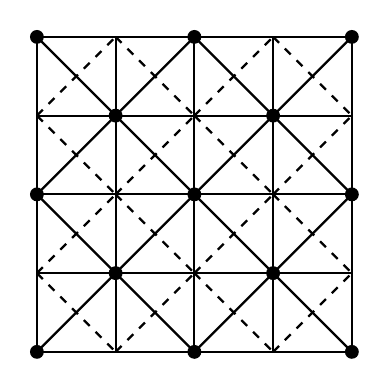
\begin{tikzpicture}[scale=1]
        % 绘制基础水平和垂直网格线
        \draw[step=1cm,black,thick] (0,0) grid (4,4);
        
        % 逐个小方格绘制对角线，避免实线和虚线重叠
        \foreach \x in {0,1,2,3} {
            \foreach \y in {0,1,2,3} {
                % 判断当前小方格左下角 (x,y) 坐标和的奇偶性
                \pgfmathparse{mod(\x+\y,2)==0}
                \ifnum\pgfmathresult=1
                    % 如果 (x,y) 是偶数点
                    % (x,y) 到 (x+1,y+1) 连结两个偶数点 -> 实线
                    \draw[thick] (\x,\y) -- (\x+1,\y+1);
                    % (x,y+1) 到 (x+1,y) 连结两个奇数点 -> 虚线
                    \draw[dashed,thick] (\x,\y+1) -- (\x+1,\y);
                \else
                    % 如果 (x,y) 是奇数点
                    % (x,y) 到 (x+1,y+1) 连结两个奇数点 -> 虚线
                    \draw[dashed,thick] (\x,\y) -- (\x+1,\y+1);
                    % (x,y+1) 到 (x+1,y) 连结两个偶数点 -> 实线
                    \draw[thick] (\x,\y+1) -- (\x+1,\y);
                \fi
            }
        }
        
        % 绘制节点（黑点和红星）
        \foreach \x in {0,1,2,3,4} {
            \foreach \y in {0,1,2,3,4} {
                \pgfmathparse{mod(\x+\y,2)==0}
                \ifnum\pgfmathresult=1
                    \fill[black] (\x,\y) circle (2.5pt);
                \else
                    % 使用略暗的红色以更贴近原图质感
                    \node[red!80!black] at (\x,\y) {\large $\bigstar$};
                \fi
            }
        }
    \end{tikzpicture}\par
    \vspace{0.5cm}
    
    % 图例部分
    \begin{tikzpicture}
        \fill[black] (0,0) circle (2.5pt) node[right=3pt, black] {偶数点};
        \node[red!80!black] at (2.5,0) {\large $\bigstar$};
        % 修正了图例中文字的颜色，原图文字为黑色
        \node[right=3pt, black] at (2.6,0) {奇数点};
    \end{tikzpicture}
    \captionof{figure}{跳点格式格点分类示意图.}
    \label{fig:跳点格式}
\end{figure}

\noindent\textbf{Step 2：在不同格点上使用不同的差分格式.} 在偶格点上使用四点显式格式离散，而奇格点上使用四点隐式格式离散.
    \begin{itemize}
        \item 当 $j+(n+1)$ 为偶数时，
        \begin{equation}\label{eq:4.6}
            \frac{u_j^{n+1}-u_j^n}{\tau}-a\frac{u_{j+1}^n-2u_j^n+u_{j-1}^n}{h^2}=0,
        \end{equation}
        \item 当 $j+(n+1)$ 为奇数时，
        \begin{equation}\label{eq:4.7}
            \frac{u_j^{n+1}-u_j^n}{\tau}-a\frac{u_{j+1}^{n+1}-2u_j^{n+1}+u_{j-1}^{n+1}}{h^2}=0.
        \end{equation}
    \end{itemize}

    注意，当 $j+n+2$ 为偶数时，由 \eqref{eq:4.6} 知
        \begin{equation}\label{eq:4.8}
            \frac{u_j^{n+2}-u_j^{n+1}}{\tau}=a\frac{u_{j+1}^{n+1}-2u_j^{n+1}+u_{j-1}^{n+1}}{h^2}.
        \end{equation}
        而当 $j+n+1$ 为奇数时，由 \eqref{eq:4.7} 知
        \begin{equation}\label{eq:4.9}
            \frac{u_j^{n+1}-u_j^n}{\tau}=a\frac{u_{j+1}^{n+1}-2u_j^{n+1}+u_{j-1}^{n+1}}{h^2}.
        \end{equation}

    根据 \eqref{eq:4.8} 和 \eqref{eq:4.9} 可以发现，当 $j+n+1$ 为奇数时，
    \begin{equation}\label{eq:4.10}
        u_j^{n+2}=2u_j^{n+1}-u_j^n,
    \end{equation}
    由此知，当 $j+n+1$ 为奇数时，跳点格式为
    \begin{equation}\label{eq:4.11}
        \frac{u_j^{n+2}-u_j^n}{2\tau}-a\frac{u_{j+1}^{n+1}-(u_j^{n+2}+u_j^n)+u_{j-1}^{n+1}}{h^2}=0.
    \end{equation}
    换言之，隐式格式 \eqref{eq:4.7} 实为显式格式 \eqref{eq:4.11}，且恰为 Dufort-Frankel 格式.

    \begin{conclusion}[小节]
        容易验证，跳点格式的精度和稳定性与 Dufort-Frankel 格式是一致的.但从计算步骤上看，已知初始格点值 $u_j^0$，可用显式格式 \eqref{eq:4.6} 算出 $n=1$ 时间层的偶格点函数值，然后再用格式 \eqref{eq:4.11} 算出奇格点上的值，该值不保存，直接由关系式 \eqref{eq:4.10} 算下一时间层的 $u_j^{n+2}$，该值保存后，用于再下一时间层的计算.继续该过程直至算出最后一个时间层的偶数格点函数值，再用隐式格式 \eqref{eq:4.11} 算出奇格点函数值.因此跳点格式虽与 Dufort-Frankel 格式等价，但节省存储和计算量.
    \end{conclusion}


\section{初边值问题第一类边值条件}

设相应的初边值问题为
\begin{equation}
    \begin{cases}
        u_t - au_{xx} = 0, \quad 0 < x < 1, \; t > 0, \\
        t=0, u = f(x), \\
        x=0, u = \varphi(t), \\
        x=1, u = \phi(t),
    \end{cases}
\end{equation}
式中 $a > 0$ 为常数.此时，差分方法的构造是常规的，给定如下：
\begin{itemize}
    \item 目标点：$(x_j, t_n)$， $x_j = jh, t_n = n\tau$，$Jh = 1, N\tau = T$.
    \item 内格点上的离散： $\dfrac{u_j^{n+1} - u_j^n}{\tau} - a \dfrac{u_{j+1}^n - 2u_j^n + u_{j-1}^n}{h^2} = 0$.
    \item 边值格点上的离散：$u_0^n = \varphi(n\tau)$， $u_J^n = \phi(n\tau)$.
    \item 初值格点上的离散：$u_j^0 = f(x_j) = f_j$.
\end{itemize}


\section{第三类边值条件}

如果对以上问题附加如下边界条件：
\begin{equation}
    \begin{cases}
        x=0 : u_x(0,t) = \alpha u(0,t) + \mu(t), \quad t > 0, \\
        x=1 : u_x(1,t) = \beta u(1,t) + \gamma(t), \quad t > 0,
    \end{cases}
\end{equation}
则内部点和初值点处的离散同上，但对于边值条件的离散要小心.
\begin{enumerate}
    \item 常规方法.
    \begin{align*}
        \frac{u_1^n - u_0^n}{h} &= \alpha u_0^n + \mu(t_n), \\
        \frac{u_J^n - u_{J-1}^n}{h} &= \beta u_J^n + \gamma(t_n).
    \end{align*}
    该格式在空间方向只有一阶精度.
    \item 虚拟格点法.为了提高边界点处的精度，将边界点往区域外延拓一个步长，即引入虚拟格点 $x_{-1}$ 和 $x_{J+1}$，然后在边界点处用中心差分离散一阶导数.为了消去虚拟点，假设方程在边界处成立，从而有
    \begin{equation}
        \begin{cases}
            \dfrac{u_1^n - u_{-1}^n}{2h} = \alpha u_0^n + \mu(t_n), \\[7pt]
            \dfrac{u_0^{n+1}-u_0^n}{\tau} - a\dfrac{u_{1}^n-2u_0^n+u_{-1}^n}{h^2} = 0,
        \end{cases}
    \end{equation}
    \begin{equation}
        \begin{cases}
            \dfrac{u_{J+1}^n - u_{J-1}^n}{2h} = \beta u_J^n + \gamma(t_n), \\[7pt]
            \dfrac{u_J^{n+1}-u_J^n}{\tau} - a\dfrac{u_{J+1}^n-2u_J^n+u_{J-1}^n}{h^2} = 0.
        \end{cases}
    \end{equation}
    由此导出二阶精度逼近方法如下：
    \begin{align*}
        u_0^{n+1} &= [1 - 2a\lambda(1 + \alpha h)]u_0^n + 2a\lambda u_1^n - 2a\lambda h\mu(t_n), \\
        u_J^{n+1} &= [1 - 2a\lambda(1 - \beta h)]u_J^n + 2a\lambda u_{J-1}^n + 2a\lambda h\gamma(t_n).
    \end{align*}

    \begin{figure}[H]
        \centering
        \begin{tikzpicture}[xscale=1.5,yscale=2]
        \draw[-stealth] (-0.7,0) -- (3.9,0) node[right] {$x$};
        \draw[-stealth] (0,0) -- (0,1.2) node[above] {$t$};
        \foreach \x in {0,0.4,...,3.2} {
             \draw (\x,0) -- (\x,1.2);
        }
        \draw[dashed] (-0.4,0) -- (-0.4,1.2);
        \draw[thick] (3.2,0) -- (3.2,1.2);
        \draw[dashed] (3.6,0) -- (3.6,1.2);
        \node[below] at (-0.4,0) {\small $x_{-1}$};
        \node[below] at (0,0) {\small $x_0$};
        \node[below] at (3.2,0) {\small $x_J$};
        \node[below] at (3.6,0) {\small $x_{J+1}$};
    \end{tikzpicture}
        \captionof{figure}{虚拟格点法求边值.}
    \end{figure}

\end{enumerate}

\section{对流扩散方程初值问题的差分格式}

我们目前已经了解了对流方程
    \begin{equation*}
        u_t + au_x = 0,
    \end{equation*}
它对应着宏观效应.同时，我们也了解了扩散方程
    \begin{equation*}
        u_t - \nu u_{xx} = 0,
    \end{equation*}
它对应着微观效应.但在科学与工程诸多领域中很多研究问题兼具宏微观效应，例如探索大气中物质浓度的扩散，海洋中水的温度变化等.如何建立相应的数学模型？

\begin{figure}[H]
    \centering
    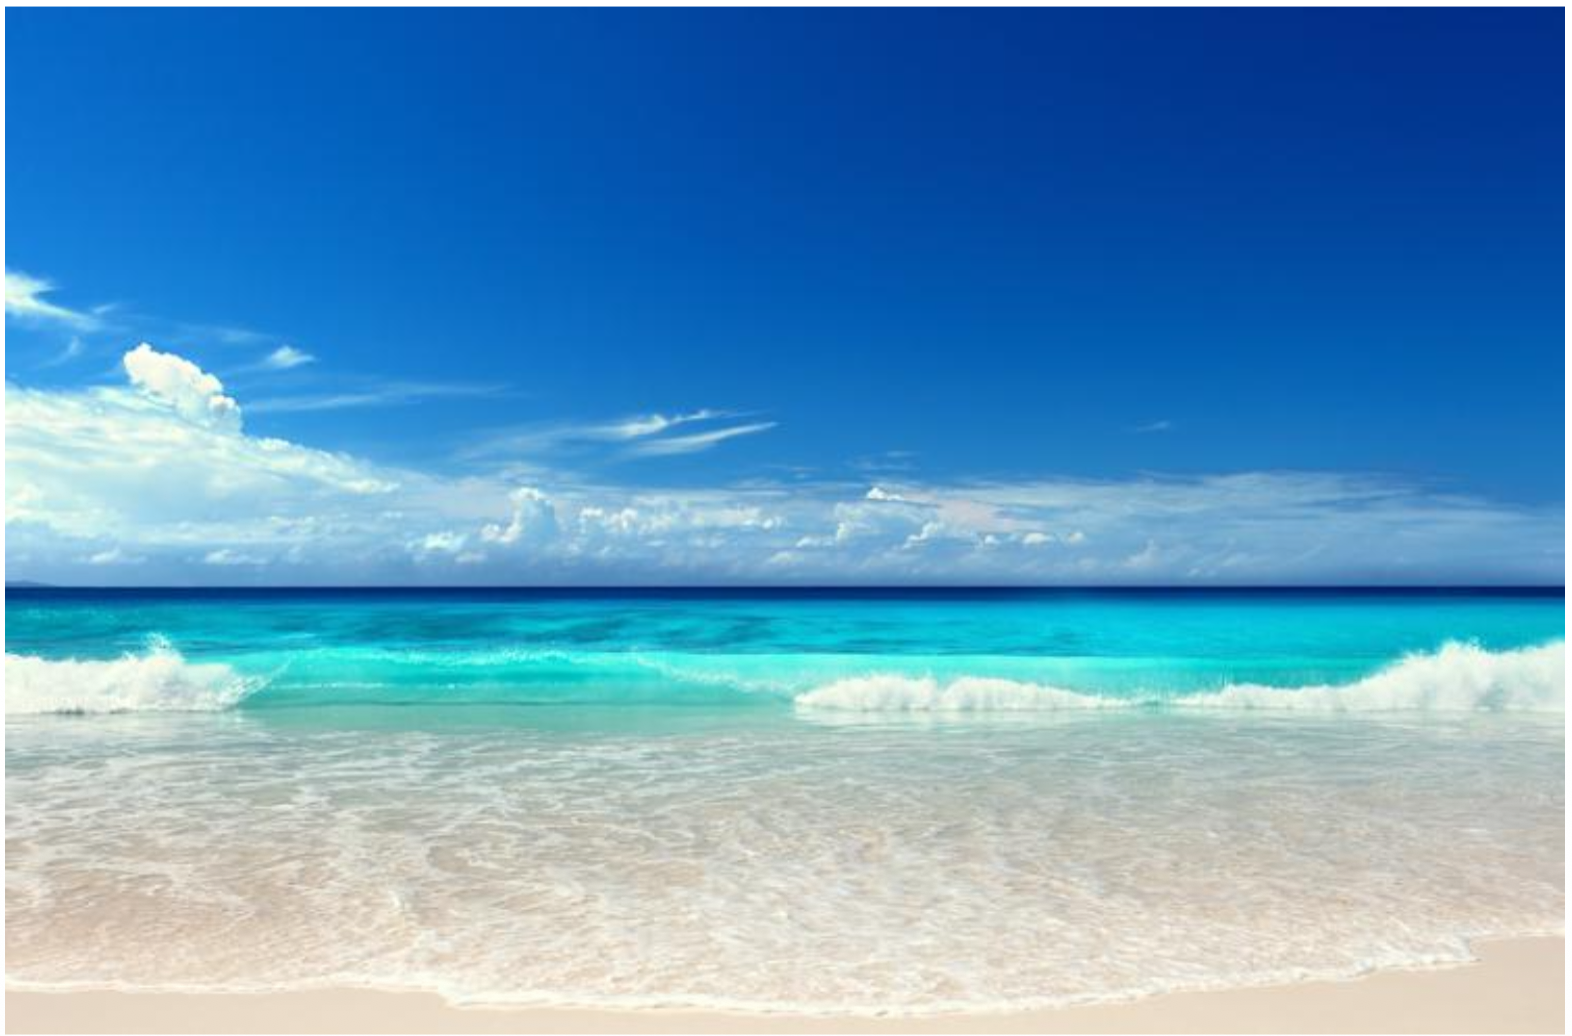
\includegraphics[width=0.6\textwidth]{fig/4.3.png}
\end{figure}

由叠加原理，可以将对流方程和扩散方程叠加在一起，得到如下的对流扩散方程：
    \begin{equation}\label{eq:对流扩散}
        \begin{cases}
            u_t + au_x = \nu u_{xx}, \quad -\infty < x < +\infty, \quad t > 0, \\
            t=0, \quad u = u_0(x),
        \end{cases}
    \end{equation}
    式中，$a, \nu > 0$ 为常数.

同样地，可以得到高维情形下的对流扩散方程：
    \begin{equation*}
        \begin{cases}
            u_t + \nabla\cdot(\bm{v}u) = \nu\Delta u, \quad \bm{x} \in \mathbb{R}^d, \quad t > 0, \\
            t=0, \quad u = u_0(\bm{x}).
        \end{cases}
    \end{equation*}




\subsection{差分格式的建立}

设欲求解的问题为对流扩散方程.

\noindent{\allbf{1. 中心差分格式}}
时间导数用向前差商离散, 空间导数用中心差商离散, 则有
\begin{equation}\label{eq:convection-diffusion-center}
    \begin{cases}
        \frac{u_j^{n+1} - u_j^n}{\tau} + a \frac{u_{j+1}^n - u_{j-1}^n}{2h} = \nu\frac{u_{j+1}^n - 2u_j^n + u_{j-1}^n}{h^2}, \\
        u_j^0 = f(x_j) = f_j.
    \end{cases}
\end{equation}
易知该格式的截断误差为 $O(\tau + h^2)$. 若令 $\lambda = a\tau/h$, $\mu = \nu\tau/h^2$, 则直接计算得差分格式对应的增长因子为
\begin{equation*}
    G(\tau, k) = 1 - 2\mu(1 - \cos kh) - \iu\lambda \sin kh,
\end{equation*}
于是
\begin{align*}
    |G(\tau, k)|^2 &= [1 - 2\mu(1 - \cos kh)]^2 + \lambda^2\sin^2 kh \\
    &= 1 - 4\mu(1 - \cos kh) + 4\mu^2(1 - \cos kh)^2 + \lambda^2\sin^2 kh \\
    &= 1 - (1 - \cos kh) \left[ 4\mu - 4\mu^2(1 - \cos kh) - \lambda^2(1 + \cos kh) \right].
\end{align*}
差分格式稳定的充要条件为 $|G(\tau, k)|^2 \leq 1$. 它等价于
\begin{equation*}
    4\mu - 4\mu^2(1 - \cos kh) - \lambda^2(1 + \cos kh) \geq 0,
\end{equation*}
即
\begin{equation*}
    (\lambda^2 - 4\mu^2)(1 - \cos kh) + 4\mu - 2\lambda^2 \geq 0, \quad \forall k \in \mathbb{R}.
\end{equation*}
注意到 $(1 - \cos kh) \in [0, 2]$, 上式等价于
\begin{equation*}
    4\mu - 2\lambda^2 \geq 0, \quad 2(\lambda^2 - 4\mu^2) + 4\mu - 2\lambda^2 \geq 0,
\end{equation*}
此即
\begin{equation}\label{eq:convection-diffusion-center-stability}
    \tau \leq \frac{2\nu}{a^2}, \quad \nu\frac{\tau}{h^2} \leq \frac{1}{2}.
\end{equation}
可以看到, 稳定性条件的第二个不等式恰是热方程向前差分格式的步长限制, 而第一项是由对流项导致的. 显然, 对流占优问题的时间步长要很小才能保证格式稳定.因此该方法更适用于扩散占优问题.

\noindent{\allbf{2. 迎风差分格式}}
类似对流方程, 我们有如下的迎风格式
\begin{equation}\label{eq:convection-diffusion-upwind}
    \frac{u_j^{n+1} - u_j^n}{\tau} + a \frac{u_j^n - u_{j-1}^n}{h} = \nu\frac{u_{j+1}^n - 2u_j^n + u_{j-1}^n}{h^2}.
\end{equation}
易知该格式的截断误差为 $O(\tau + h)$. 稳定性可类似前面分析, 一个更简单的方法是把上式写为中心差分格式的形式, 即
\begin{equation*}
    \frac{u_j^{n+1} - u_j^n}{\tau} + a \frac{u_{j+1}^n - u_{j-1}^n}{2h} = \left(\nu + \frac{ah}{2}\right)\frac{u_{j+1}^n - 2u_j^n + u_{j-1}^n}{h^2}.
\end{equation*}
令 $\bar{\nu} = \nu + \frac{ah}{2}$, 则由上一格式的稳定性分析知稳定性条件为
\begin{equation*}
    \tau \leq \frac{2\bar{\nu}}{a^2}, \quad \bar{\nu}\frac{\tau}{h^2} \leq \frac{1}{2},
\end{equation*}
即
\begin{equation*}
    \tau \leq \frac{2}{a^2} \left(\nu + \frac{ah}{2}\right), \quad \left(\nu + \frac{ah}{2}\right)\frac{\tau}{h^2} \leq \frac{1}{2}.
\end{equation*}
若把第一个式子写为第二个的形式, 则有
\begin{align*}
    \left(\nu + \frac{ah}{2}\right)\frac{\tau}{h^2} &\leq \frac{2}{a^2h^2}\left(\nu + \frac{ah}{2}\right)^2 = 2\left(\frac{\nu}{ah} + \frac{1}{2}\right)^2 \\
    &= \frac{1}{2} + 2\left(\frac{\nu^2}{a^2h^2} + \frac{\nu}{ah}\right),
\end{align*}
而第二个式子比它的要求更强, 因此迎风格式的稳定性条件为
\begin{equation}\label{eq:convection-diffusion-upwind-stability}
    \left(\nu + \frac{ah}{2}\right)\frac{\tau}{h^2} \leq \frac{1}{2}.
\end{equation}
正因为对流项的系数乘以了空间步长 $h$, 从稳定性角度来说, 若 $a$ 比 $\nu$ 大很多, 即对流占优情形时, 差分格式的时间步长不需要选取特别小.

\noindent{\allbf{3. 隐式格式}}
Crank-Nicolson 型的隐式差分格式为
\begin{align}\label{eq:convection-diffusion-cn}
    \frac{u_j^{n+1} - u_j^n}{\tau} &+ \frac{a}{2} \left( \frac{u_{j+1}^n - u_{j-1}^n}{2h} + \frac{u_{j+1}^{n+1} - u_{j-1}^{n+1}}{2h} \right) \notag \\
    = \frac{\nu}{2} &\left( \frac{u_{j+1}^n - 2u_j^n + u_{j-1}^n}{h^2} + \frac{u_{j+1}^{n+1} - 2u_j^{n+1} + u_{j-1}^{n+1}}{h^2} \right),
\end{align}
其截断误差为 $O(\tau^2 + h^2)$. 格式的增长因子为
\begin{equation*}
    G(\tau, k) = \frac{(1 - \mu + \mu\cos kh) - \iu\frac{\lambda}{2}\sin kh}{(1 + \mu - \mu\cos kh) + \iu\frac{\lambda}{2}\sin kh},
\end{equation*}
式中 $\lambda, \mu$ 同中心差分格式. 于是
\begin{equation*}
    |G(\tau, k)|^2 = \frac{(1 - \mu + \mu\cos kh)^2 + \left(\frac{\lambda}{2}\sin kh\right)^2}{(1 + \mu - \mu\cos kh)^2 + \left(\frac{\lambda}{2}\sin kh\right)^2}.
\end{equation*}
经计算有 $|G(\tau, k)| \leq 1$, 从而\textcolor{red}{隐式差分格式无条件稳定}.

\section{变系数方程 Taylor 展开法和有限体积法}

设欲求解的问题为如下抛物型方程
\begin{equation}\label{eq:variable-coeff-parabolic}
    \begin{cases}
        u_t - a(x)u_{xx} = 0, \\
        t=0,u=u_0(x),
    \end{cases}
\end{equation}
的初值问题, 其中$a(x)$ 是一个充分光滑函数, 且存在常数 $a_0 > 0$ 使得对任意 $x \in \mathbb{R}$, $a(x) \geq a_0 > 0$.

\subsection{Taylor 展开法}


\begin{note}[Taylor展开法核心思想]
\begin{itemize}
    \item 离散和连续的转换, 时间求导和空间求导的转换.
    \item Taylor 展开.
\end{itemize}
\end{note}

引入中心差商算子 $\delta_x^2 u = [u(x+h, t) - 2u(x,t) + u(x-h, t)]/h^2$. 则由 Taylor 展开和方程 \eqref{eq:variable-coeff-parabolic} 知
\begin{align*}
    \delta_x^2 u &= u_{xx} + \frac{h^2}{12} u_{xxxx} + O(h^4) \\
    &= \frac{1}{a} u_t + \frac{1}{12} \left(\frac{1}{a} u_t\right)_{xx} + O(h^4).
\end{align*}
再使用中心差分离散可得
\begin{align*}
    (\delta_x^2 u)_j &= \left(\frac{1}{a} u_t\right)_j + \frac{h^2}{12} \delta_x^2 \left(\frac{1}{a} u_t\right)_j + O(h^4) \\
    &= \frac{5}{6} \left(\frac{1}{a} u_t\right)_j + \frac{1}{12} \left(\frac{1}{a} u_t\right)_{j+1} + \frac{1}{12} \left(\frac{1}{a} u_t\right)_{j-1} + O(h^4).
\end{align*}
如果在 $n+1/2$ 时间步对 $u_t$ 离散且采用 Crank-Nicolson 格式的思想构造差分方程, 则由上式立得以下格式:
\begin{equation}\label{eq:compact-cn}
    \frac{1}{12} \frac{u_{j+1}^{n+1} - u_{j+1}^n}{a_{j+1}\tau} + \frac{5}{6} \frac{u_j^{n+1} - u_j^n}{a_j\tau} + \frac{1}{12} \frac{u_{j-1}^{n+1} - u_{j-1}^n}{a_{j-1}\tau} = \frac{(\delta_x^2 u)_j^{n+1} + (\delta_x^2 u)_j^n}{2}.
\end{equation}
由构造易知该格式的截断误差为 $O(\tau^2 + h^4)$.使用能量方法可以证明该格式无条件稳定.\par
格式 \eqref{eq:compact-cn} 实即紧致的 Crank-Nicolson 格式, 它也可以如下导出. 在点 $(x_j, t_{n+1/2})$ 处考虑微分方程 \eqref{eq:variable-coeff-parabolic}, 有
\begin{equation*}
    u_t(x_j, t_{n+1/2}) = a_j u_{xx}(x_j, t_{n+1/2}).
\end{equation*}
然后在时间方向采用 Crank-Nicolson 格式的构造思想, 而得
\begin{equation*}
    \delta_t u_j^{n+1/2} = \frac{1}{2} [a_j u_{xx}(x_j, t_n) + a_j u_{xx}(x_j, t_{n+1})],
\end{equation*}
式中 $\delta_t v^{n+1/2} = \frac{1}{\tau}(v^{n+1} - v^n)$. 或等价地,
\begin{equation*}
    \frac{u_j^{n+1} - u_j^n}{a_j\tau} = \frac{1}{2} [u_{xx}(x_j, t_n) + u_{xx}(x_j, t_{n+1})].
\end{equation*}
在空间方向对以上方程两边作用紧致差分算子 $\mathcal{W}_x$, 由紧致差分格式的类似推导即可得差分格式 \eqref{eq:compact-cn}.

\subsection{有限体积法}

接着, 来考虑如下抛物型方程:
\begin{equation}\label{eq:variable-coeff-parabolic-divergence}
    u_t = (a(x)u_x)_x
\end{equation}
的初值问题的数值求解, 式中 $a(x)$ 仍然是一个充分光滑函数, 且存在常数 $a_0 > 0$ 使得对任意 $x \in \mathbb{R}$, $a(x) \geq a_0 > 0$. \par
使用有限体积法来构造差分格式. \par
\noindent\allbf{Step1.将\eqref{eq:variable-coeff-parabolic-divergence}写为一阶方程组} 设$w = a(x)u_x$.则方程 \eqref{eq:variable-coeff-parabolic-divergence} 为
\begin{equation}\label{eq:variable-coeff-system}
    \begin{cases}
        u_t - w_x = 0,\\
        w=a(x)u_x.
    \end{cases}
\end{equation}
\noindent\allbf{Step2.使用控制体积得格式}
对于网格点 $(x_j, t_n)$, 取有限体积元为
\begin{equation*}
    W = \{ (x,t) : t_n < t < t_{n+1}, x_{j-1/2} < x < x_{j+1/2} \}.
\end{equation*}
对 \eqref{eq:variable-coeff-system} 在 $W$ 上积分并使用牛顿-莱布尼茨公式有
\begin{align}\label{eq:finite-volume-integral}
    0 &= \iint_W (u_t - w_x) \,\mathrm{d}x\mathrm{d}t \notag \\
    &= \int_{x_{j-1/2}}^{x_{j+1/2}} \int_{t_n}^{t_{n+1}} (u_t - w_x) \,\mathrm{d}t \mathrm{d}x \notag \\
    &= \int_{x_{j-1/2}}^{x_{j+1/2}} [u(x, t_{n+1}) - u(x, t_n)] \,\mathrm{d}x - \int_{t_n}^{t_{n+1}} [w(x_{j+1/2}, t) - w(x_{j-1/2}, t)] \,\mathrm{d}t \notag \\
    &=: I_1 - I_2.
\end{align}
对于 $I_1$, 由数值积分的中矩形公式知
\begin{equation}\label{eq:I1-approx}
    I_1 \approx [u(x_j, t_{n+1}) - u(x_j, t_n)]h.
\end{equation}
对于 $I_2$ 的进一步离散更有技巧性. 首先, 由$w=a(x)u_x$有
\begin{equation*}
    a^{-1}(x)w = u_x.
\end{equation*}
对其关于 $x$ 由 $x_j$ 到 $x_{j+1}$ 积分知
\begin{equation*}
    u(x_{j+1}, t) - u(x_j, t) = \int_{x_j}^{x_{j+1}} a^{-1}(x)w(x,t) \,\mathrm{d}x \approx w(x_{j+1/2}, t) \int_{x_j}^{x_{j+1}} a^{-1}(x) \,\mathrm{d}x.
\end{equation*}
从而推得
\begin{equation}\label{eq:5.8}
    w(x_{j+1/2}, t) \approx \frac{u(x_{j+1}, t) - u(x_j, t)}{\int_{x_j}^{x_{j+1}} a^{-1}(x) \,\mathrm{d}x} = \frac{u(x_{j+1}, t) - u(x_j, t)}{h} A_{j+1},
\end{equation}
式中，
\begin{equation*}
    A_{j+1} = h\left(\int_{x_j}^{x_{j+1}} a^{-1}(x) \,\mathrm{d}x\right)^{-1}.
\end{equation*}

另一方面，由数值积分的广义梯形公式知
\begin{equation}\label{eq:5.9}
    \int_{t_n}^{t_{n+1}} w(x_{j+1/2}, t) \,\mathrm{d}t \approx [(1 - \theta)w(x_{j+1/2}, t_n) + \theta w(x_{j+1/2}, t_{n+1})] \tau,
\end{equation}
式中 $\theta \in [0, 1]$. 因此，由 \eqref{eq:5.8} 和 \eqref{eq:5.9} 可以得到 $I_2$ 的逼近. 将该结果和 \eqref{eq:I1-approx} 代入 \eqref{eq:finite-volume-integral} 可得
\begin{align*}
    \frac{u(x_j, t_{n+1}) - u(x_j, t_n)}{\tau} - \frac{1}{h^2} [\theta \Delta (A_j\nabla u(x_j, t_{n+1})) + (1 - \theta)\Delta (A_j\nabla u(x_j, t_n))] \approx 0,
\end{align*}
式中
\begin{equation*}
    \Delta u(x_j, t_n) = u(x_{j+1}, t_n) - u(x_j, t_n), \quad \nabla u(x_j, t_n) = u(x_j, t_n) - u(x_{j-1}, t_n)
\end{equation*}
分别是一阶向前差分和向后差分.

以上结果写成差分方程即
\begin{equation}\label{eq:5.10}
    \frac{u_j^{n+1} - u_j^n}{\tau} - \frac{1}{h^2} [\theta \Delta (A_j\nabla u_j^{n+1}) + (1 - \theta)\Delta (A_j\nabla u_j^n)] = 0.
\end{equation}

当 $\theta = 1/2$ 时，该格式的精度为 $O(\tau^2 + h^2)$，而当 $\theta \neq 1/2$ 时，该格式的精度为 $O(\tau + h^2)$.\par
当$A_j$为常数时，上述格式即为古典隐式格式.\par

\begin{remark}
在热物理中，$u$ 表示温度场，而 $w$ 为负热流量，它们均为空间位置的连续函数，而对于界面问题 $u_x$ 可能是非连续函数，因此使用积分方式得到 $w(x_{j+1/2}, t)$ 近似值适用性更广.
\end{remark}

\section{二维抛物方程差分法：一维问题的直接推广}

\subsection{显式和隐式格式}

考虑问题
\begin{equation}\label{eq:6.1}
    \begin{cases}
        u_t = a\Delta u = a(u_{xx} + u_{yy}), \quad (x, y) \in \Omega = (0, 1) \times (0, 1), \quad t > 0, \\
        t = 0, \quad u = f(x, y), \quad (x, y) \in \Omega, \\
        u = 0, \quad (x, y) \in \partial\Omega,
    \end{cases}
\end{equation}
式中 $a > 0$ 为常数. 设网格剖分的格点为 $(x_j, y_l, t_n)$，其中 $x_j = jh$, $y_l = lh$, $t_n = n\tau$，$Jh = 1$, $Lh = 1$. 引入记号
\begin{equation*}
    \delta_x^2 u_{jl}^n = \frac{u_{j+1,l}^n - 2u_{jl}^n + u_{j-1,l}^n}{h^2}, \quad \delta_y^2 u_{jl}^n = \frac{u_{j,l+1}^n - 2u_{jl}^n + u_{j,l-1}^n}{h^2}.
\end{equation*}

类似一维问题，我们可以直接给出 \eqref{eq:6.1} 的显式格式
\begin{equation*}
    \frac{u_{jl}^{n+1} - u_{jl}^n}{\tau} = a\left(\delta_x^2 u_{jl}^n + \delta_y^2 u_{jl}^n\right)
\end{equation*}


由于是常系数问题，因此仍可应用Fourier方法研究其稳定性条件.对于二维问题，为了获得增长因子，可令
\begin{equation*}
    u_{jl}^n = v^n e^{\iu(k_1 jh + k_2 lh)},
\end{equation*}
其中 $\boldsymbol{k} = (k_1, k_2)$ 为波数. 将其代入显式格式
\begin{equation}\label{eq:6-exp-scheme}
    \frac{u_{jl}^{n+1} - u_{jl}^n}{\tau} = a\left(\delta_x^2 u_{jl}^n + \delta_y^2 u_{jl}^n\right),
\end{equation}
首先计算 $x$ 方向的二阶中心差分：
\begin{align*}
    \delta_x^2 u_{jl}^n
    &= \frac{u_{j+1,l}^n - 2u_{jl}^n + u_{j-1,l}^n}{h^2} \\
    &= \frac{v^n e^{\iu(k_1 (j+1)h + k_2 lh)} - 2v^n e^{\iu(k_1 jh + k_2 lh)} + v^n e^{\iu(k_1 (j-1)h + k_2 lh)}}{h^2} \\
    &= \frac{v^n e^{\iu(k_1 jh + k_2 lh)}\bigl(e^{\iu k_1 h} - 2 + e^{-\iu k_1 h}\bigr)}{h^2} \\
    &= u_{jl}^n \cdot \frac{2\cos(k_1 h) - 2}{h^2}
     = -u_{jl}^n \cdot \frac{4\sin^2 \frac{k_1 h}{2}}{h^2}.
\end{align*}
同理可得 $y$ 方向的二阶中心差分：
\begin{equation*}
    \delta_y^2 u_{jl}^n = -u_{jl}^n \cdot \frac{4\sin^2 \frac{k_2 h}{2}}{h^2}.
\end{equation*}
记网格比 $\lambda = \tau / h^2$，将以上两式代入显式格式 \eqref{eq:6-exp-scheme}：
\begin{align*}
    u_{jl}^{n+1}
    &= u_{jl}^n + a\tau\bigl(\delta_x^2 u_{jl}^n + \delta_y^2 u_{jl}^n\bigr) \\
    &= u_{jl}^n - a\tau \cdot u_{jl}^n \left(\frac{4\sin^2 \frac{k_1 h}{2}}{h^2} + \frac{4\sin^2 \frac{k_2 h}{2}}{h^2}\right) \\
    &= u_{jl}^n \left[1 - 4a\lambda\left(\sin^2 \frac{k_1 h}{2} + \sin^2 \frac{k_2 h}{2}\right)\right].
\end{align*}
将 $u_{jl}^n = v^n e^{\iu(k_1 jh + k_2 lh)}$ 和 $u_{jl}^{n+1} = v^{n+1} e^{\iu(k_1 jh + k_2 lh)}$ 代入上式，消去公共因子 $e^{\iu(k_1 jh + k_2 lh)}$，得到
\begin{equation*}
    v^{n+1} = G(\tau, \boldsymbol{k}) v^n,
\end{equation*}
式中增长因子为
\begin{equation}\label{eq:6-growth}
    G(\tau, \boldsymbol{k}) = 1 - 4a\lambda \left(\sin^2 \frac{k_1 h}{2} + \sin^2 \frac{k_2 h}{2}\right).
\end{equation}

格式稳定的充要条件是 $|G(\tau, \boldsymbol{k})| \leq 1$ 对一切 $\boldsymbol{k} \in \mathbb{R}^2$ 成立，即
\begin{equation*}
    -1 \leq 1 - 4a\lambda\left(\sin^2 \frac{k_1 h}{2} + \sin^2 \frac{k_2 h}{2}\right) \leq 1.
\end{equation*}
右端不等式 $1 - 4a\lambda(\sin^2 \frac{k_1 h}{2} + \sin^2 \frac{k_2 h}{2}) \leq 1$ 自然成立. 左端不等式给出
\begin{equation*}
    4a\lambda\left(\sin^2 \frac{k_1 h}{2} + \sin^2 \frac{k_2 h}{2}\right) \leq 2,
\end{equation*}
即
\begin{equation*}
    a\lambda \leq \frac{1}{2\left(\sin^2 \frac{k_1 h}{2} + \sin^2 \frac{k_2 h}{2}\right)}.
\end{equation*}
因此稳定性条件为$a\lambda \leq \frac{1}{4}.$\par
同样地，我们可以直接求解方程的隐式格式\begin{equation}\label{eq:6.2}
    \frac{u_{jl}^{n+1} - u_{jl}^n}{\tau} = a\left(\delta_x^2 u_{jl}^{n+1} + \delta_y^2 u_{jl}^{n+1}\right).
\end{equation}
对于隐式格式 \eqref{eq:6.2}，用同样方法可得其增长因子为
\begin{equation*}
    G(\tau, \boldsymbol{k}) = \frac{1}{1 + 4a\lambda\left(\sin^2 \frac{k_1 h}{2} + \sin^2 \frac{k_2 h}{2}\right)},
\end{equation*}
显然对任意 $\lambda > 0$ 均有 $0 < G \leq 1$，故隐式格式是无条件稳定的.\par
将稳定性条件推广到 $d$ 维空间中, 显式格式的稳定性条件为 $2a\lambda\cdot d \leq 1$, 而隐式格式仍然是无条件稳定的.



\begin{remark}[困难]
\begin{itemize}
    \item 二维问题的显式格式比一维问题的时间步长约束更强. 隐式格式尽管是无条件稳定的，但系数矩阵不再是三对角的，而是五对角的，计算量也大大高于显式格式. 可见，在二维情形，显格式和隐格式都不方便.
    \item 因此，构造计算量不大且保持无条件稳定的差分格式具有重要的理论意义和应用价值.
\end{itemize}
\end{remark}

\section{交替方向隐式格式}

采用二步思想，构造Peaceman-Rachford格式.

\begin{itemize}
    \item 使用时间方向分数步思想，引入 $n + 1/2$ 层过渡时间层.
    \item 在 $n \rightarrow n + 1/2$ 层对 $u_{xx}$ 隐式离散，$u_{yy}$ 显式离散. 在 $n + 1/2 \rightarrow n + 1$ 层对 $u_{yy}$ 隐式离散，$u_{xx}$ 显式离散.
\end{itemize}

\begin{equation}\label{eq:7.1-7.2}
    \begin{cases}
        \frac{u_{jl}^{n+1/2} - u_{jl}^n}{\tau/2} = a\left(\delta_x^2 u_{jl}^{n+1/2} + \delta_y^2 u_{jl}^n\right), \quad \text{在 } x \text{ 方向求解}, &(1)\\[7pt]
        \frac{u_{jl}^{n+1} - u_{jl}^{n+1/2}}{\tau/2} = a\left(\delta_x^2 u_{jl}^{n+1/2} + \delta_y^2 u_{jl}^{n+1}\right), \quad \text{在 } y \text{ 方向求解}. &(2) 
    \end{cases}
\end{equation}

\begin{figure}[H]
    \centering
    \begin{tikzpicture}[scale=0.8]
        % Bottom layer (n)
        \draw (0,0) -- (2,1) -- (4,1) -- (2,0) -- cycle;
        \draw[dashed] (1,0.5) -- (3,0.5);
        \draw[dashed] (1.5,0.25) -- (2.5,0.75);
        \fill (2,0.5) circle (2pt) node[right, font=\footnotesize] {};
        \fill (1,0.5) circle (2pt);
        \fill (3,0.5) circle (2pt);
        \node at (5, 0.5) {\footnotesize $n$层};

        % Middle layer (n+1/2)
        \begin{scope}[yshift=1.5cm]
            \draw (0,0) -- (2,1) -- (4,1) -- (2,0) -- cycle;
            \draw[dashed] (1,0.5) -- (3,0.5);
            \draw[dashed] (1.5,0.25) -- (2.5,0.75);
            \fill (2,0.5) circle (2pt);
            \fill (1.5,0.25) circle (2pt);
            \fill (2.5,0.75) circle (2pt);
            \node at (5, 0.5) {\footnotesize $n+\frac{1}{2}$层};
            \draw[thick] (1.5,0.25) -- (2.5,0.75);
        \end{scope}

        % Top layer (n+1)
        \begin{scope}[yshift=3cm]
            \draw (0,0) -- (2,1) -- (4,1) -- (2,0) -- cycle;
            \draw[dashed] (1,0.5) -- (3,0.5);
            \draw[dashed] (1.5,0.25) -- (2.5,0.75);
            \fill (2,0.5) circle (2pt);
            \fill (1,0.5) circle (2pt);
            \fill (3,0.5) circle (2pt);
            \node at (5, 0.5) {\footnotesize $n+1$层};
            \draw[thick] (1,0.5) -- (3,0.5);
        \end{scope}
        
        % Thick lines on bottom layer
        \draw[thick] (1,0.5) -- (3,0.5);

        % Vertical dashed line connecting centers
        \draw[dashed] (2,0.5) -- (2,3.5);

        % Axes
        \begin{scope}[xshift=-1cm, yshift=1cm]
            \draw[->] (0,0) -- (1,0) node[right] {$y$};
            \draw[->] (0,0) -- (-0.8,-0.6) node[left] {$x$};
        \end{scope}
    \end{tikzpicture}
    \caption{交替方向隐式格式示意图}
\end{figure}

对于$(1)$，
\begin{equation*}
    \frac{v^{n+1/2}-v^n}{\tau /2}=\frac{a}{h^2}\ab(-4\sin^2\frac{k_1h}{2}v^{n+1/2}-4\sin^2\frac{k_2h}{2}v^n)
\end{equation*}
即
\begin{equation*}
    \ab(1+2a\lambda\sin^2\frac{k_1h}{2})v^{n+1/2}=\ab(1-2a\lambda\sin^2\frac{k_2h}{2})v^n.
\end{equation*}
故
\begin{equation*}
    v^{n+1/2}=\frac{1-2a\lambda\sin^2\frac{k_2h}{2}}{1+2a\lambda\sin^2\frac{k_1h}{2}}v^n.
\end{equation*}

同理，对于$(2)$，我们有
\begin{equation*}
    v^{n+1}=\frac{1-2a\lambda\sin^2\frac{k_1h}{2}}{1+2a\lambda\sin^2\frac{k_2h}{2}}v^{n+1/2}.
\end{equation*}

消去 $u_{jl}^{n+1/2}$，有
\begin{equation*}
    v^{n+1}=\frac{(1-2a\lambda\sin^2\frac{k_1h}{2})(1-2a\lambda\sin^2\frac{k_2h}{2})}{(1+2a\lambda\sin^2\frac{k_1h}{2})(1+2a\lambda\sin^2\frac{k_2h}{2})}v^n.
\end{equation*}
故$v^{n+1} = G(\tau, \boldsymbol{k})v^n$，式中
\begin{equation*}
    G(\tau, \boldsymbol{k}) = \frac{(1 - 2a\lambda\sin^2\frac{k_1h}{2})(1 - 2a\lambda\sin^2\frac{k_2h}{2})}{(1 + 2a\lambda\sin^2\frac{k_1h}{2})(1 + 2a\lambda\sin^2\frac{k_2h}{2})}.
\end{equation*}
易知 $|G(\tau, \boldsymbol{k})| \leq 1$，因此该格式是无条件稳定的. 另外，利用 Taylor 展开可知该方法的精度为 $O(\tau^2 + h^2)$.

\begin{remark}[小节]
降维的技巧加上分数步技巧. 该格式计算量较小且无条件稳定. 另外需要注意的是，若将 PR 格式 \eqref{eq:7.1-7.2} 推广到三维问题时，相应的格式不再是无条件稳定的.
\end{remark}

\section{算子分裂方法}

\subsection{从一个简单例子谈起}

\begin{note}[历史回顾]
分数步方法是求解多维复杂问题的经济且有效的方法. 早在 1971 年，苏联数学家 Yanenko 就在其专著中对该方法进行了系统性的论述. 前面介绍了求解抛物型方程的交替方向隐式差分格式，就是一种分数步格式. 这一节我们将介绍另一种分数步方法，与交替方向隐式格式不同的是，该方法在每一步仅处理发展方程右端的一个算子，因而称为算子分裂方法. 其实算子分裂方法有多种类型，这里只介绍其中的一种.
\end{note}

考虑问题
\begin{equation}\label{eq:8.1}
    \begin{cases}
        \frac{\mathrm{d}x}{\mathrm{d}t} = f(t) = 1, \quad 0 < t \leq T, \\
        x(0) = 0.
    \end{cases}
\end{equation}
将区间 $[0, T]$ 作 $N$ 等分，得如下格点：
\begin{equation*}
    0 = t_0 < t_1 < \cdots < t_n < t_{n+1} < \cdots < t_N = T,
\end{equation*}
式中，$t_n = n\tau$，而 $\tau$ 为步长. 对时间剖分的每一个固定子区间 $[t_n, t_{n+1}]$，我们将给出 \eqref{eq:8.1} 在该区间上的一个分数步近似.

注意到
\begin{equation*}
    x(t_n) = \sum_{i=0}^{n-1} \int_{t_i}^{t_{i+1}} f(s) \,\mathrm{d}s = \sum_{i=0}^{n-1} \int_{t_i}^{t_{i+1}} 1 \,\mathrm{d}s, \quad n = 1, \dots, N.
\end{equation*}

显然，若把每个小区间 $[t_n, t_{n+1}]$ 上对 $f$ 的积分作用等效在该时间段的前半部分，则格点上的计算结果不变，此时 $f(\tau, t)$ 在 $[t_n, t_{n+1}]$ 的取值为
\begin{equation}\label{eq:8.2}
    f(\tau, t) = \begin{cases}
        2, & t_n < t \leq t_{n+1/2}, \\
        0, & t_{n+1/2} < t \leq t_{n+1},
    \end{cases}
\end{equation}
式中，$t_n = n\tau$，$t_{n+1/2} = (n+1/2)\tau$.

记 $x_\tau(t)$ 为如下问题之解：
\begin{equation}\label{eq:8.3}
    \begin{cases}
        \frac{\mathrm{d}x_\tau}{\mathrm{d}t} = f_\tau(t) = f(\tau, t), \quad 0 < t \leq T, \\
        x_\tau(0) = 0,
    \end{cases}
\end{equation}
式中 $f(\tau, t)$ 由 \eqref{eq:8.2} 确定. 该问题的等价描述为
\begin{equation}\label{eq:8.4}
    \begin{cases}
        \frac{\mathrm{d}x_\tau}{\mathrm{d}t} = 2, \quad n\tau < t \leq (n+\frac{1}{2})\tau, \\[7pt]
        \frac{\mathrm{d}x_\tau}{\mathrm{d}t} = 0, \quad (n+\frac{1}{2})\tau < t \leq (n+1)\tau.
    \end{cases}
\end{equation}

直观上，当 $\tau \rightarrow 0+$ 时，近似解 $x_\tau$ 应该在某种意义下收敛到精确解 $x$. 具体而言，对任意的 $0 \leq t_* < t^* \leq T$，有
\begin{equation*}
    x(t^*) = x(t_*) + \int_{t_*}^{t^*} f(s) \,\mathrm{d}s.
\end{equation*}
这样，对步长为 $\tau$ 的时间划分，如果 $f(t)$ 的近似 $f(\tau, t)$ 能在积分意义下收敛，即
\begin{equation}\label{eq:8.5}
    \int_{t_*}^{t^*} [f(\tau, s) - f(s)] \,\mathrm{d}s \rightarrow 0, \quad \tau \rightarrow 0+ \quad \forall\ 0 \leq t_* < t^* \leq T,
\end{equation}
那么近似问题的解 $x_\tau(t)$ 必逐点收敛于 $x(t)$. 我们称在 \eqref{eq:8.5} 的意义下，$f(\tau, t)$ 弱收敛于 $f(t)$. 可以证明，\eqref{eq:8.2} 给出的 $f(\tau, t)$ 弱收敛于 $f(t) \equiv 1$.

在以下示意图中，给出了函数 $f(t)$ 和它的近似 $f(\tau, t)$，以及相应解 $x(t)$ 和近似解 $x_\tau(t)$ 的图形描述，佐证了以上理论分析的正确性.

\begin{figure}[H]
    \centering
    % 定义与原图相近的颜色
\definecolor{myorange}{RGB}{218,128,72}
\definecolor{myblue}{RGB}{70,105,185}

\begin{tikzpicture}[
    >=Latex,
    axis/.style={thick, -stealth, >=Latex},
    dashline/.style={densely dashed, myblue, thin},
    orangeline/.style={thick, myorange},
    blackline/.style={thick, black},
    scale=0.8
]

% ==================== 左图 (f vs t) ====================
\begin{scope}[xshift=0cm]
    % 绘制坐标轴
    \draw[axis] (0,0) -- (6.8,0) node[right] {$t$};
    \draw[axis] (0,0) -- (0,4.2) node[left] {$f$};

    % Y轴刻度与标签
    \node[left] at (0,0) {0};
    \node[left] at (0,1.5) {1};
    \node[left] at (0,3) {2};

    % X轴刻度与标签
    \node[below=2pt] at (0,0) {$t_0$};
    \node[below=2pt, myorange] at (1,0) {$t_{1/2}$};
    \node[below=2pt] at (2,0) {$t_1$};
    \node[below=2pt, myorange] at (3,0) {$t_{3/2}$};
    \node[below=2pt] at (4,0) {$t_2$};
    \node[below=2pt, myorange] at (5,0) {$t_{5/2}$};
    \node[below=2pt] at (6,0) {$t_3$};

    % 蓝色虚线参考线
    \foreach \x in {1,2,3,4,5,6} {
        \draw[dashline] (\x,0) -- (\x,3);
    }

    % 绘制 f(t) = 1 (黑色水平线)
    \draw[blackline] (0,1.5) -- (6.5,1.5) node[right] {$f(t) \equiv 1$};

    % 绘制 f(tau, t) (橙色阶跃函数)
    \draw[orangeline] (0,3) -- (1,3);
    \draw[orangeline] (1,0) -- (2,0);
    \draw[orangeline] (2,3) -- (3,3);
    \draw[orangeline] (3,0) -- (4,0);
    \draw[orangeline] (4,3) -- (5,3);
    \draw[orangeline] (5,0) -- (6,0);

    % 函数标签
    \node[above] at (1.5, 3.2) {$f(\tau,t)$};
\end{scope}

% ==================== 右图 (x vs t) ====================
\begin{scope}[xshift=9cm] % 向右平移以便并排显示
    % 绘制坐标轴
    \draw[axis] (0,0) -- (6.8,0) node[right] {$t$};
    \draw[axis] (0,0) -- (0,4.2) node[left] {$x$};

    % X轴刻度与标签 (与左图一致)
    \node[below=2pt] at (0,0) {$t_0$};
    \node[below=2pt, myorange] at (1,0) {$t_{1/2}$};
    \node[below=2pt] at (2,0) {$t_1$};
    \node[below=2pt, myorange] at (3,0) {$t_{3/2}$};
    \node[below=2pt] at (4,0) {$t_2$};
    \node[below=2pt, myorange] at (5,0) {$t_{5/2}$};
    \node[below=2pt] at (6,0) {$t_3$};

    % 蓝色虚线参考线
    \draw[dashline] (1,0) -- (1,1);
    \draw[dashline] (2,0) -- (2,1);
    \draw[dashline] (3,0) -- (3,2);
    \draw[dashline] (4,0) -- (4,2);
    \draw[dashline] (5,0) -- (5,3);
    \draw[dashline] (6,0) -- (6,3);

    % 绘制 x(t) (黑色直线)
    \draw[blackline] (0,0) -- (6,3) node[right=2mm] {$x(t)$};

    % 绘制 x_tau(t) (橙色折线)
    \draw[orangeline] (0,0) -- (1,1) -- (2,1) -- (3,2) -- (4,2) -- (5,3) -- (6,3);

    % 函数标签
    \node[above left] at (4.1, 2.7) {$x_\tau(t)$};
\end{scope}

\end{tikzpicture}
    \caption{$f(t), x(t)$ 和 $f(\tau, t), x_\tau(t)$ 的比较}
\end{figure}

\begin{note}[启示]
\begin{itemize}
    \item 为了求解问题 \eqref{eq:8.1}，可以转而求解近似问题 \eqref{eq:8.3} 或它的等价问题 \eqref{eq:8.4}. 而构造近似问题 \eqref{eq:8.3} 的关键是在每个子区间 $[t_n, t_{n+1}]$ 如何合理修改右端函数.
    \item 从力学直观上看，如果将 $f(t)$ 理解为时刻 $t$ 受到的力，那么若时间步长 $\tau$ 很小时，它在 $[t_n, t_{n+1}]$ 的作用效应应和由 \eqref{eq:8.2} 给定的力 $f(\tau, t)$ 的作用效应差不多.
\end{itemize}
\end{note}

\subsection{一般化及在抛物型方程中的应用}

\begin{remark}[一般化]
如果系统受到多个力的作用，$f(t) = f_1(t) + \cdots + f_p(t)$，可以定义
\begin{equation*}
    f(\tau, t) = p f_i(t), \quad t_{n+(i-1)/p} < t \leq t_{n+i/p}, \quad i = 1, \dots, p,
\end{equation*}
转而求解近似问题
\begin{equation*}
    \begin{cases}
        \frac{\mathrm{d}x_\tau}{\mathrm{d}t} = f_\tau(t) = f(\tau, t), \quad 0 < t \leq T, \\
        x_\tau(0) = 0.
    \end{cases}
\end{equation*}
或等价地，
\begin{equation*}
    \frac{\mathrm{d}x_\tau}{\mathrm{d}t} = p f_i(t), \quad t_{n+(i-1)/p} < t \leq t_{n+i/p}, \quad i = 1, \dots, p.
\end{equation*}
于是，在每个子区间 $[t_{n+(i-1)/p}, t_{n+i/p}]$ 上，只需求解受到单个人力 $f_i(t)$ 作用的问题，从而可能将原问题转化为另一个便于处理的近似问题，达到\textbf{分而治之}的目的. 这正是算子分裂法思想的精髓.
\end{remark}

现在来考虑一般的初值问题
\begin{equation}\label{eq:8.6}
    \begin{cases}
        u_t = Lu, \quad t \in (0, T], \\
        t = 0, \ u = u_0(x),
    \end{cases}
\end{equation}
式中
\begin{equation*}
    L = L_1 + L_2 + \cdots + L_p.
\end{equation*}
仿照上面的思想，可构造如下算子
\begin{equation*}
    L_\tau = \alpha_1(\tau, t)L_1 + \alpha_2(\tau, t)L_2 + \cdots + \alpha_p(\tau, t)L_p,
\end{equation*}
式中，
\begin{equation*}
    \alpha_s(\tau, t) = p \delta_{si}, \quad t_{n+(i-1)/p} < t \leq t_{n+i/p},
\end{equation*}
\begin{equation*}
    \delta_{si} = \begin{cases}
        1, & s = i, \\
        0, & s \neq i.
    \end{cases}
\end{equation*}
于是算子分裂方法的思想就是将原问题 \eqref{eq:8.6} 转化为以下问题的求解
\begin{equation*}
    \frac{\partial u_\tau}{\partial t} = L_\tau u_\tau.
\end{equation*}
写成子区间描述的形式，上即
\begin{equation*}
    \frac{\partial u_\tau}{\partial t}(t) = p L_i u_\tau(t), \quad t_{n+(i-1)/p} < t \leq t_{n+i/p}, \quad i = 1, \dots, p.
\end{equation*}

\subsection{算子分裂方法在抛物型方程差分方法中的应用}

\begin{note}[算子分裂方法实施步骤]
\begin{itemize}
    \item 首先，通过算子分裂技巧获得原问题的可分步求解近似问题.
    \item 然后再对相应的子问题使用合理的数值方法进行离散，最终获得求解原问题的高效数值方法.
\end{itemize}
\end{note}

考虑二维抛物型方程
\begin{equation*}
    \frac{\partial u}{\partial t} = a\left(\frac{\partial^2 u}{\partial x^2} + \frac{\partial^2 u}{\partial y^2}\right).
\end{equation*}
记
\begin{equation*}
    L_1 u = a \frac{\partial^2 u}{\partial x^2}, \quad L_2 u = a \frac{\partial^2 u}{\partial y^2}.
\end{equation*}
根据前面的讨论，分裂格式相当于在 $[t_n, t_{n+1}]$ 考虑如下问题的求解
\begin{equation*}
    \begin{cases}
        \frac{\partial u_\tau}{\partial t} = 2L_1 u_\tau = 2a \frac{\partial^2 u_\tau}{\partial x^2}, & t_n < t \leq t_{n+1/2}, \\[7pt]
        \frac{\partial u_\tau}{\partial t} = 2L_2 u_\tau = 2a \frac{\partial^2 u_\tau}{\partial y^2}, & t_{n+1/2} < t \leq t_{n+1}.
    \end{cases}
\end{equation*}

如果采用 Crank-Nicholson 差分格式求解相应的子问题（一维抛物型方程），则最终获得如下的局部一维格式:
\begin{equation*}
    \begin{cases}
        \frac{1}{2} \frac{u_{jl}^{n+1/2} - u_{jl}^n}{\tau/2} = a\delta_x^2 \dfrac{u_{jl}^{n+1/2} + u_{jl}^n}{2}, \\[6pt]
        \frac{1}{2} \frac{u_{jl}^{n+1} - u_{jl}^{n+1/2}}{\tau/2} = a\delta_y^2 \dfrac{u_{jl}^{n+1} + u_{jl}^{n+1/2}}{2}.
    \end{cases}
\end{equation*}
在本格式中，$x$ 和 $y$ 方向采用了相同的步长 $h$ 进行网格剖分，相异步长的格式类似可知.

我们还可以把算子分裂方法导出的差分格式与预测-校正方法相结合，得到精度更高的格式. 预测-校正方法的思想是首先用一个精度不是很高但计算简单的格式获得粗糙的结果，然后用精度较高的格式对该结果进行校正.

这样，我们可对 $[t_n, t_{n+1}]$ 的前半部分采用分裂格式获得 $u_{jl}^{n+1/2}$，然后用精度较高的 Crank-Nicolson 格式校正，从而获得如下的预测-校正格式:
\begin{equation}\label{eq:8.7}
    \begin{cases}
        \left.\begin{aligned}
            \frac{u_{jl}^{n+1/4} - u_{jl}^n}{\tau/2} = a\delta_x^2 u_{jl}^{n+1/4} \\
            \frac{u_{jl}^{n+1/2} - u_{jl}^{n+1/4}}{\tau/2} = a\delta_y^2 u_{jl}^{n+1/2}
        \end{aligned}\right\} \Rightarrow \text{预测}, \\
        \frac{u_{jl}^{n+1} - u_{jl}^n}{\tau} = a(\delta_x^2 + \delta_y^2)u_{jl}^{n+1/2} \Rightarrow \text{校正}.
    \end{cases}
\end{equation}

借助算子分裂方法，可以构造三维抛物型方程的无条件稳定的差分格式. 例如，考虑如下三维抛物型方程
\begin{equation*}
    u_t=a\Delta u = au_{xx} + au_{yy} + au_{zz}.
\end{equation*}
则相应的分裂格式为
\begin{equation*}
    \begin{cases}
        (u_\tau)_t=3a(u_\tau)_{xx},t_n<t\leq t_{n+1/3}, \\
        (u_\tau)_t=3a(u_\tau)_{yy},t_{n+1/3}<t\leq t_{n+2/3}, \\
        (u_\tau)_t=3a(u_\tau)_{zz},t_{n+2/3}<t\leq t_{n+1}.
    \end{cases}
\end{equation*}

在本节中，主要研究了求解高维抛物型方程算子分裂方法的构造，实际上，使用相同的思想也可以构造求解高维双曲型方程算子分裂方法. 考虑到方法的构造思想是完全相同的，我们就在此不展开讨论了.






